% CREATED BY MAGNUS GUSTAVER, 2020

\ifx\ThesisType\undefined
Undefined Thesis type in settings.tex
\else
  \if\ThesisType M
    \else
    \if\ThesisType B
    \else
    Define \textbackslash ThesisType as M for master's thesis or B for bachelor thesis in settings.tex
    \fi
  \fi
\fi

% COVER PAGE
\begin{titlepage}
\newgeometry{top=3cm, bottom=1cm,
			left=2.25 cm, right=2.25cm}	% Temporarily change margins		
			
%Header Front Page
\ifx\ThesisType\undefined
\else
    \if\ThesisType M
    \vtop{
        \null\vspace{-25mm}
        \centerline{
\includegraphics[width=1.18\textwidth]{figure/auxiliary/GrayHeaderPattern.jpg}}
        \vspace{-2.3cm}
        \hbox{\hspace{0mm}
\includegraphics[height=18mm]{figure/auxiliary/AvancezChalmersU_white_right.eps}}
        \centerline{\textcolor{headerBrown}{\rule{1.18\textwidth}{4pt}}}
        \vspace{\paperheight}\vspace{-85mm}
        \centerline{\textcolor{thesisHeaderColor}{\rule{1.1\textwidth}{0.8pt}}} % Rule after Department
        \vspace{-\paperheight}\vspace{85mm}
    }
    \fi
    \if\ThesisType B
    \vtop{
        \null\vspace{-25mm}
        \centerline{
\includegraphics[width=1.18\textwidth,height=80pt]{figure/auxiliary/GreenHeaderPattern.jpg}}
        \vspace{-2.0cm}
        \centerline{\hbox{\hspace{0mm}
\includegraphics[height=12mm]{figure/auxiliary/banner_logo.eps}}}
        % {figure/auxiliary/AvancezChalmers_white_right.eps}
        \vspace{0.3cm}
        \centerline{\textcolor{headerBrown}{\rule{1.18\textwidth}{4pt}}}
        \vspace{\paperheight}\vspace{-85mm}
        \centerline{\textcolor{thesisHeaderColor}{\rule{1.1\textwidth}{0.8pt}}} % Rule after Department
        \vspace{-\paperheight}\vspace{85mm}
    }
    \fi
\fi

% Cover picture (replace with your own or delete)		
% \begin{figure}[H]
% \centering
% \vspace{1cm}	% Adjust vertical spacing here
% 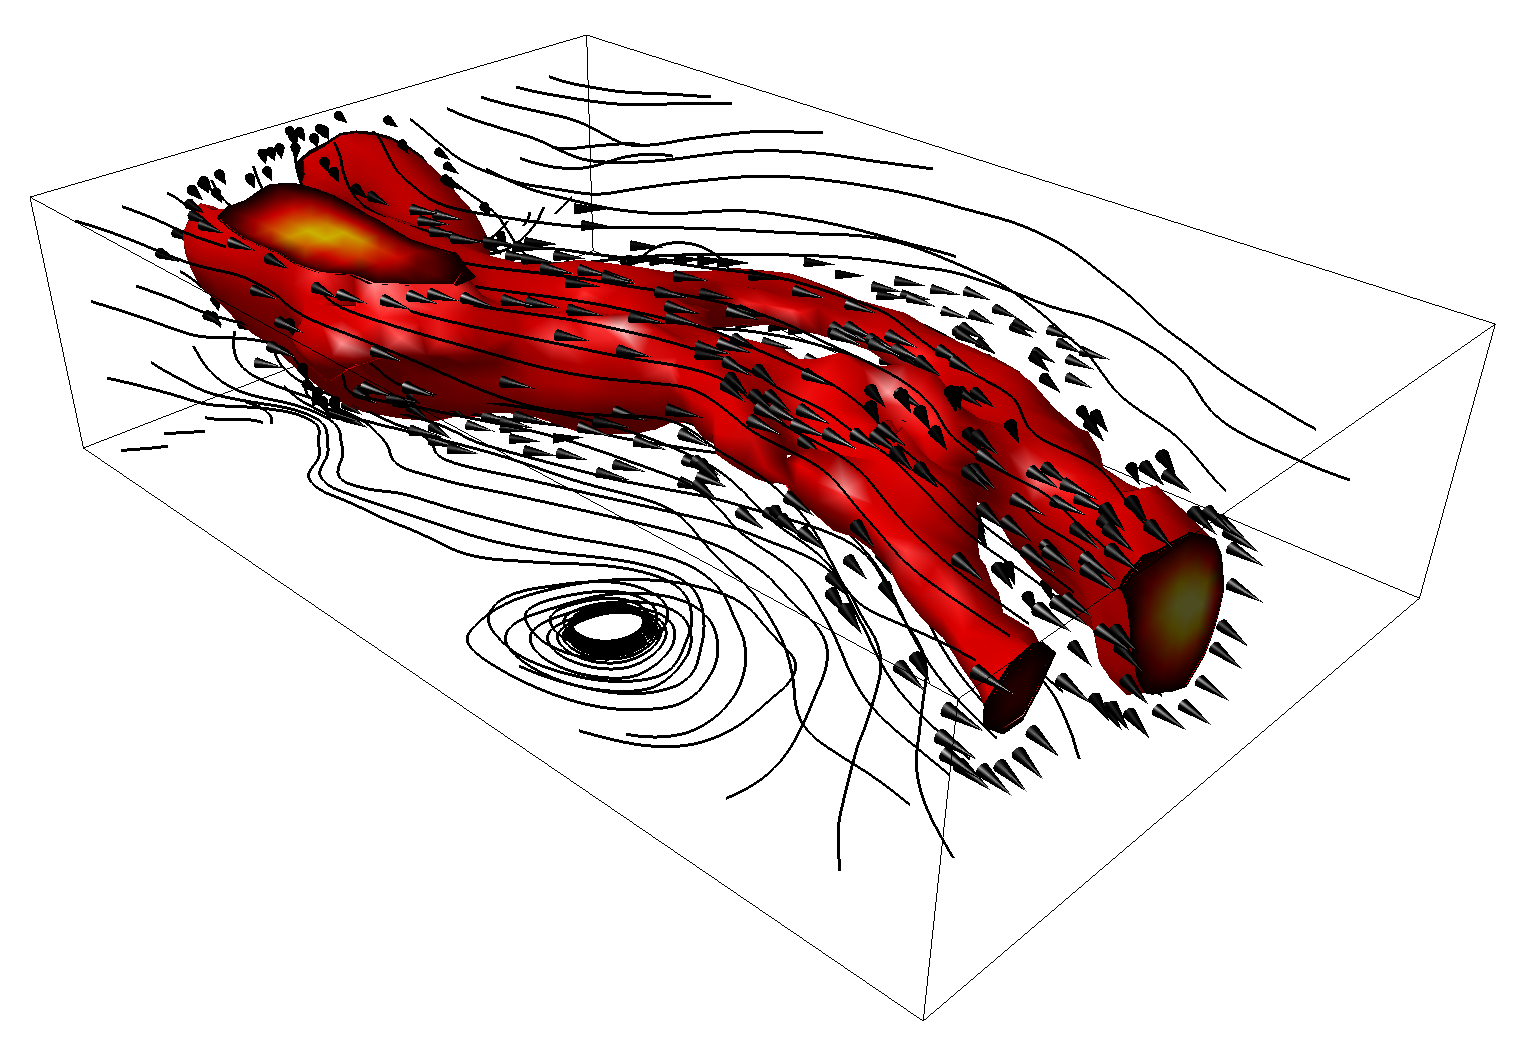
\includegraphics[width=0.9\linewidth]{figure/Wind.png}
% \end{figure}

% Cover text
\mbox{}
\vfill
\renewcommand{\familydefault}{\sfdefault} \normalfont % Set cover page font
\textbf{{\Huge 	Creating a programming language
                based on System F}} 	\\[0.5cm]
{\Large If suggest we skip this subtitle}\\[0.5cm]
Bachelor's thesis DATX11-VT23-66 \setlength{\parskip}{1cm}

\noindent
{\Large
    Victor Olin\\[2mm]
    Martin Fredin\\[2mm]
    Samuel Hammersberg\\[2mm]
    William Bodin\\[2mm]
    Sebastian Selander\\[2mm]
    Valter Miari}\setlength{\parskip}{0.5cm}\\
% \hspace{0cm}
% {\Large Martin Fredin} \setlength{\parskip}{1.5cm}\\
% {\Large Samuel Hammersberg} \setlength{\parskip}{1.5cm}\\
% {\Large William Bodin} \setlength{\parskip}{1.5cm}\\
% {\Large Sebastian Selander} \setlength{\parskip}{1.5cm}\\
% {\Large Valter Miari} \setlength{\parskip}{1.5cm}\\

\noindent
\textcolor{thesisHeaderColor}{\small\textbf{DEPARTMENT OF COMPUTER SCIENCE AND ENGINEERING}}
\setlength{\parskip}{1mm}

\textsc{Chalmers University of Technology} \\
\textsc{University of Gothenburg} \\
{\small Gothenburg, Sweden \the\year \\
\href{www.chalmers.se}{www.chalmers.se}}\vspace{1.2cm}

\renewcommand{\familydefault}{\rmdefault} \normalfont % Reset standard font
\end{titlepage}


% BACK OF COVER PAGE (BLANK PAGE)
\newpage
\restoregeometry
\thispagestyle{empty}
\mbox{}


% TITLE PAGE
\newpage
\thispagestyle{empty}
\begin{center}
	\textsc{\large Bachelor's thesis \the\year}\\[4cm]
	\textbf{\Large Creating a programming language based on System F} \\[1cm]
	% {\large A Subtitle that can be Very Much Longer if Necessary}\\[1cm]
	{\large Victor Olin}\\[1mm]
	{\large Martin Fredin}\\[1mm]
	{\large Samuel Hammersberg}\\[1mm]
	{\large William Bodin}\\[1mm]
	{\large Sebastian Selander}\\[1mm]
	{\large Valter Miari}
	
	\vfill	
	% Logotype on titlepage	
	\begin{figure}[H]
	\centering
	% Remove this figure to remove the titlepage logotype
	\if\ThesisType M
    
\includegraphics[width=0.2\pdfpagewidth]{figure/auxiliary/AvancezChalmersU_black_centered.eps} \\
    \fi
    \if\ThesisType B
    
\includegraphics[width=0.23\pdfpagewidth]{figure/auxiliary/cth_uog_logo.eps} \\
    \fi
	% 
\includegraphics[width=0.2\pdfpagewidth]{figure/auxiliary/AvancezChalmersU_black_centered.eps} \\
	\end{figure}	\vspace{5mm}	
	
	Department of Computer Science and Engineering \\
	% \emph{Division of Division name}\\
	% Name of research group (if applicable)\\
	\textsc{Chalmers University of Technology} \\
	\textsc{University of Gothenburg} \\
	Gothenburg, Sweden \the\year \\
\end{center}


% IMPRINT PAGE (BACK OF TITLE PAGE)
\newpage
\thispagestyle{plain}
\vspace*{4.5cm}
Creating a programming language based on System F\\
% A Subtitle that can be Very Much Longer if Necessary\\
\setlength{\parskip}{1cm}

\copyright ~ Victor Olin, Martin Fredin, Samuel Hammersberg, William Bodin, Sebastian Selander, Valter Miari \the\year. \setlength{\parskip}{1cm}

Supervisor: Patrik Jansson, Computing Science division, Department of Computer Science and Engineering\\
Examiner: Alex Gerdes, Computing Science division, Department of Computer Science and Engineering \setlength{\parskip}{1cm}

Bachelor's Thesis \the\year\\	
Department of Computer Science and Engineering\\
% Division of Division name\\
% Name of research group (if applicable)\\
Chalmers University of Technology\\
% University of Gothenburg\\
SE-412 96 Gothenburg\\
Telephone +46 31 772 1000 \setlength{\parskip}{0.5cm}

\vfill
% Caption for cover page figure if used, possibly with reference to further information in the report
% Cover: Wind visualization constructed in Matlab showing a surface of constant wind speed along with streamlines of the flow. \setlength{\parskip}{0.5cm}

Typeset in \LaTeX \tagtemp\\
Printed by Chalmers Reproservice\\
Gothenburg, Sweden \the\year
